\documentclass[../main.tex]{subfiles}

\begin{document}

Diana es una comerciante exitosa que se caracteriza por utilizar métodos estadísticos como soporte a la toma de decisiones. En esta ocasión, ella realizó un estudio con el propósito de predecir el valor total de las ventas mensuales (variable aleatoria $Y$), en millones de pesos, utilizando los gastos en publicidad mensual, en millones de pesos, como la variable dependiente $X$. Para ello, recolectó información de 12 sucursales de empresas similares. A continuación se presenta el resumen de los datos obtenidos por el comerciante:

\bigskip
\hrule
\begin{align*}
	n &= 12 & \bar{X} &= 34.17 & \bar{Y} = 453.75 \\
	\sum_{i = 1}^{n} y_{i}^2 &= 2512925 & 	\sum_{i = 1}^{n} x_{i}^2 &= 15650 & \sum_{i = 1}^{n} y_{i}x_{i} &= 191325
\end{align*}
\hrule
\bigskip

\begin{enumerate}[(a)]

\item \textbf{(2 puntos)}  Escriba el modelo de regresión lineal que le permite predecir el valor total de las ventas semanales en función de la publicidad semanal.

El modelo de regresión lineal simple, para la situación en cuestión, consiste en predecir (o modelar) las ventas mensuales, haciendo uso del gasto mensual de publicidad. Es decir, usando el modelo algebraico de una ecuación de primer orden, cuyo significado geométrico es una linea recta en $\mathbb{R}2$, se desea interpretar la significancia de la variable $X$ para determinar el comportamiento de la variable $Y$. Lo que se desea, es hallar los valores $\beta_0$ y $\beta_1$ en la siguiente ecuación:
$$\hat{y} = \beta_0 + \beta_0 x + \epsilon$$
Donde $\hat{y}$ representa la variable aleatoria $Y$ y $x$ la variable aleatoria $X$, y $\epsilon$ el error aleatorio.

\item \textbf{(4 puntos)}  Utilizando el método de mínimos cuadrados ordinarios, encuentre de manera teórica la ecuación para estimar los coeficientes del modelo de regresión lineal planteado en el literal $a$.

Las suposiciones generales para el desarrollo analítico del modelo son:
\begin{align*}
	\mathbb{E}(\epsilon_i) &= 0 & Var(\epsilon_i) &= \sigma ^2 & Cov(\epsilon_i, \epsilon_j) &= 0 & \forall i, j = 1, 2, ..., n \wedge i \neq j
\end{align*}
$$
\mathbb{E}(\hat{y}) = \mathbb{E}(\beta_0 + \beta_1 x + \epsilon) = \beta_0 + \beta_1 x 
$$

El método de mínimos cuadrados, minimiza la suma de los cuadrados de las desviaciones de las observaciones y el promedio de las mismas. Es decir:
$$\epsilon = y - \hat{y} = y - (\beta_0 + \beta_1 x)$$
$$\sum{i = 1}^{n} \epsilon_i ^2 = \sum_{i = 1}^{n}\left( y_i - \beta_0 + \beta_1 x_i\right) ^2$$

Para obtener los estimadores $\beta_0$, $\beta_1$, se diferencia esta última expresión con respecto a cada uno de estos y se iguala la derivada parcial a cero.

$$\frac{\partial \sum e_i^2}{\partial \beta_0} = -2 \times \left[\sum_{i = 1}^{n}\left( y_i - \hat{\beta}_0 + \hat{\beta}_1 x_i\right)\right] = 0$$
$$\frac{\partial \sum e_i^2}{\partial \beta_1} = -2 \times \left[\sum_{i = 1}^{n}x_i \times\left( y_i - \hat{\beta}_0 + \hat{\beta}_1 x_i\right)\right] = 0$$

A partir de esto, se obtienen las siguientes expresiones:
\begin{align*}
	\sum_{i = 1}^{n} y_i &= n\hat{\beta}_0 + \hat{\beta}_1 \sum_{i = 1}^{n} x_i &   	\sum_{i = 1}^{n} x_iy_i &= \hat{\beta}_0 \sum_{i = 1}^{n} x_i + \hat{\beta}_1 \sum_{i = 1}^{n} x_i^2
\end{align*}
$$\frac{\sum_{i = 1}^{n} y_i}{n} = \hat{\beta}_0 + \hat{\beta}_1 \frac{\sum_{i = 1}^{n} x_i}{n} \Rightarrow \hat{\beta}_0 = \frac{\sum_{i = 1}^{n} y_i}{n} - \hat{\beta}_1 \frac{\sum_{i = 1}^{n} x_i}{n} = \bar{y} - \hat{\beta}_1 \bar{x}$$

Al sustituir $\hat{\beta_0}$ en:
$$\sum_{i = 1}^{n} x_iy_i = \hat{\beta}_0 \sum_{i = 1}^{n} x_i + \hat{\beta}_1 \sum_{i = 1}^{n} x_i^2$$
Se obtiene:
$$\sum_{i = 1}^{n} x_iy_i = \left( \frac{\sum_{i = 1}^{n} y_i}{n} - \hat{\beta}_1 \frac{\sum_{i = 1}^{n} x_i}{n}\right) \times \sum_{i = 1}^{n} x_i + \hat{\beta}_1 \sum_{i = 1}^{n} x_i^2$$

Por lo tanto, hallar $\beta_0$ y $\beta_1$  es ahora trivial.

$$\beta_1 = \frac{\sum_{i = 1}^{n} x_iy_i - \frac{\left( \sum_{i=1}^{n} x_i\right) \times \left(\sum_{i=1}^{n} y_i \right)}{n}}{\sum_{i=1}^{n} x_i^2 - \frac{\left( \sum_{i=1}^{n} x_i\right)^2}{n}}$$
$$\beta_0 = \bar{Y} - \beta_1 \bar{X}$$

\item \textbf{(4 puntos)} Estime los parámetros del modelo de regresión lineal simple planteado en el literal $a$. Realice una interpretación de cada uno de los coeficientes estimados.

Al multiplicar por $n$, se facilita el cálculo de la expresión:
$$\beta_1 = \frac{12(191325) - 12(34.17)(473.75)}{12(15650) - (34.17  \times 12)^2} = 3.1544$$
$$\beta_0 = \bar{Y} - \beta_1 \bar{X} = 345.96$$

Se puede concluir, que los gastos de publicidad influyen de manera positiva sobre las ventas de la compañía, esto a través de los coeficientes estimados en el literal anterior. Es decir, a mayores gastos en publicidad, mayores serán las ventas.

\item \textbf{(2 puntos)} Estime la tabla ANOVA correspondiente al modelo de regresión lineal simple planteado en el litera $a$.

$$SCE = 6338.438 \wedge SCT = \sum_{i = 1}^{n} y_i ^2 - \frac{\left(\sum_{i = 1}^{n} y_i\right)}{n} \wedge SCT = SCR + SCT$$
$$SCR = 2512925 - 453.75 = 2512471.25 \Rightarrow SCT  = 2518809.688$$

\bigskip
\begin{tabular}{ |p{2cm}||p{2.5cm}|p{1cm}|p{2cm}|p{1.8cm}|  }
 \hline
 \multicolumn{5}{|c|}{ANOVA} \\
 \hline
 Model & Sum of squares & gl & Mean Square & F\\
 \hline
 Regression   & 2512471.25    &1&   $MCR_{reg}$ & $\frac{MCR_{reg}}{\left( \frac{\Sigma \left( y_i - \hat{y}_i\right)^2}{10}\right)}$\\
 Residual   & 6338.438    &10&   $\frac{\Sigma \left( y_i - \hat{y}_i\right)^2}{10}$ &\\
 Total   & 2518809.688    &11&   $\frac{\Sigma \left( y_i - \bar{y}\right)^2}{11}$ &\\
 \hline
\end{tabular}

\item \textbf{(2 puntos)} Plantee las hipótesis nula y alterna de la prueba de significancia global. Defina el estadístico de prueba y concluya en términos del contexto del problema; utilice el criterio del p-valor.
\begin{align*}
	H_0 : \beta_1 &= 0 & H_1 : \beta_1 \neq 0
\end{align*}

$$\textbf{EP} : \frac{SCR}{\left( SCE / (n - 2)\right)} \sim F(1, 11) = \frac{2512471.25}{(6338.438)/10}$$

\begin{figure}[h]
\centering
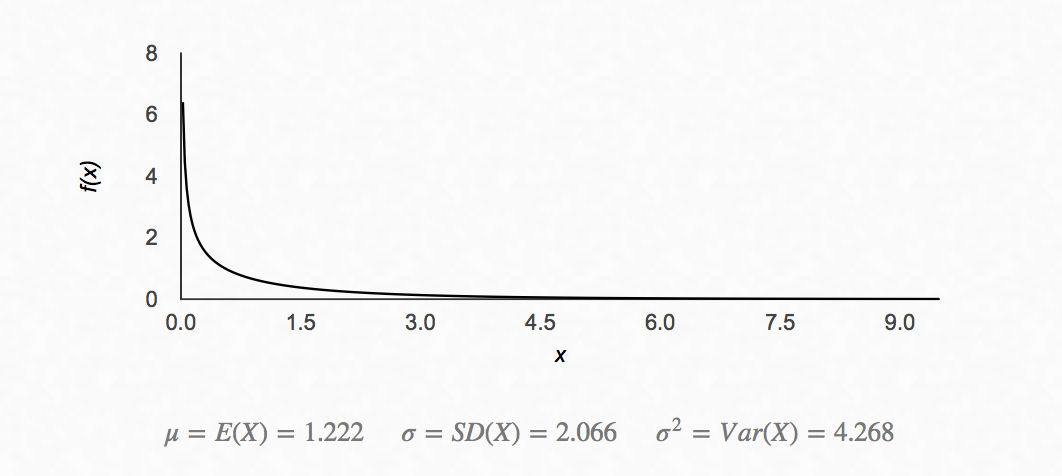
\includegraphics[width=10cm]{fdistr.png}
\label{fig:img1}
\end{figure}

Claramente, el estadístico de prueba está en la cola derecha, es decir, se rechaza la hipótesis nula.

\item \textbf{(1 punto)} Estime el valor del coeficiente de determinación, e interprételo.

$$R^2 = \frac{SCR}{SCT} \in \left[0, 1\right] \Rightarrow R^2 = \frac{2512471.25}{2518809.688} = 0.9974$$

Dado que $R^2$ es muy cercano a uno, se concluye que el modelo es globalmente sinificativo para explicar o predecir la variable $y$ haciendo uso de $x$.

\item \textbf{(16 puntos)} Plantee una prueba de significancia individual para el intercepto y para la pendiente. Para cada una, plantee las hipótesis nula y alterna y defina el estadístico de
prueba y concluya en términos del contexto del problema; utilice el criterio del p-valor.

Para $\beta_1$

\begin{align*}
	H_0 : \beta_1 &= 0 & H_1 : \beta_1 \neq 0
\end{align*}

$$\textbf{EP} = t_0 = \frac{\hat{\beta}_1 - \beta_1}{S/\sqrt{s_{xx}}} \wedge S = \sqrt{\frac{s_{yy} - \hat{\beta}_1 s_{xy}}{n-2}}$$
$$s_{xy} = \sum_{i =1}^{n}x_iy_i-n\bar{x}\bar{y} = 5269.4 \wedge s_{yy} = \sum_{i = 1}^{n}y_i^2 - n \bar{y}^2 = 42256.28$$
$$S = 50.63$$
$$s_{xx} = \sum_{i=1}^{n}x_{i}^2 - n\bar{x}^2 = 1638.93$$

El estadístico de prueba:

$$t_0 = \frac{\hat{\beta}_1 - \beta_1}{\frac{S}{\sqrt{s_{xx}}}} = 2.52$$

La región de rechazo está dada por:

$$t_0 < t_{(0.025, 10)} = -2.228 \vee t_0 > t_{(0.975, 10)} = 2.228$$

Conclusión:

Debido a que $t_0$ cae en la región de rechazo, se rechaza la hipótesis nula y se concluye que $\beta_1$ es distinto a cero.

Para $\beta_0$

\begin{align*}
	H_0 : \beta_0 &= 0 & H_1 : \beta_0 \neq 0
\end{align*}

$$\textbf{EP} = t_0 = \frac{\hat{\beta}_0 - \beta_0}{S/\sqrt{\frac{\sum{i = 1}^{n}x_i^2}{n\times s_{xx}}}} = 7.66$$

La región de rechazo está dada por:

$$t_0 < t_{(0.025, 10)} = -2.228 \vee t_0 > t_{(0.975, 10)} = 2.228$$

Conclusión:

Debido a que $t_0$ cae en la región de rechazo, se rechaza la hipótesis nula y se concluye que $\beta_0$ es distinto a cero.

\item \textbf{(8 puntos)} Calcule un intervalo de confianza ($\alpha = 0.05$) para el intercepto y para el coeficiente asociado a la variable independiente. Interprete cada uno de los intervalos.

Para $\beta_1$

$$\hat{\beta}_1 \pm t_{(\alpha / 2, 10)}\left( \frac{S}{\sqrt{s_{xx}}}\right) \Rightarrow 3.1544 \pm 2.228 \times \left( \frac{50.63}{\sqrt{1638.93}}\right)$$

$$\textbf{IC} : \left[5.94, 0.37 \right]$$

Para $\beta_0$

$$\hat{\beta}_1 \pm t_{(\alpha / 2, 10)}S\left( \sqrt{\frac{\sum_{i = 1}^{n}x_i^2}{ns_{xx}}}\right) \Rightarrow 345.96 \pm 2.228\left(50.63 \sqrt{\frac{15650}{12 \times 1638.93}}\right)$$

$$\textbf{IC} : \left[446.58, 245.334 \right]$$

\item \textbf{(4 puntos)} Diana decidió invertir 40 millones de pesos en publicidad, y las ventas mensuales fueron de 480 millones de pesos. ¿Cuál es el valor que Diana había pronosticado para las ventas? ¿Cuál es el residuo asociado a este pronóstico?

Dado que $y = 345.96 + 3.1544\times x $. Entonces el valor de ventas asociado a $40$ como gastos de publicidad es: $345.96 + 3.1544 \times 40 = 472.13$. El error residual $\epsilon$ es $480 - 472.13 = 7.87$

\end{enumerate}
\end{document}
